\section{Results}
\label{sec:results}
Spectrum regularization fails the prespecified criterion on both datasets. On TCGA-UT the tuned arm gains nothing over cohort whitening at five patients per class (0.00 points, 95\% interval: $-0.01$ to 0.00), and on BRACS $-0.11$ points ($-0.51$ to 0.20); neither reaches the one-point threshold, and neither interval lies above zero (Table~\ref{tab:accuracy}). The tuned arm is not merely flat but nearly identical to its host, because validation selects the uncompressed spectrum $\beta=1$ in 29 of 30 TCGA-UT fits at five patients, in which case the arm copies the cohort-whitening record. Compression in the direction the over-dispersion argument suggests is harmful throughout on TCGA-UT: $-0.16$ points at $\beta=0.75$, $-0.42$ at $\beta=0.5$, $-0.77$ at $\beta=0.25$, and $-0.92$ at $\beta=0$, every interval below zero. On BRACS every power arm lies within 0.35 points of cohort whitening with intervals that include zero, which is unsurprising there, since cohort whitening itself gains only 0.32 points ($-0.36$ to 1.22) over the real cohort on that dataset.

\begin{table}[htbp]
\centering
\small
\renewcommand{\arraystretch}{1.15}
\begin{tabular}{@{}lrrr@{}}
\toprule
Arm family & $G=5$ & $G=10$ & $G=20$ \\
\midrule
\multicolumn{4}{@{}l}{\emph{TCGA-UT}}\\
Real cohort (R) & 62.48 [61.24, 63.65] & 67.79 [66.47, 69.00] & 71.89 [70.55, 73.06] \\
Flat spectrum, $\beta=0$ (F) & 63.82 [62.56, 64.98] & 68.32 [67.01, 69.52] & 72.04 [70.71, 73.23] \\
$\beta=0.25$ (Ba) & 63.97 [62.73, 65.12] & 68.62 [67.31, 69.83] & 72.41 [71.06, 73.59] \\
$\beta=0.5$ (Bb) & 64.32 [63.09, 65.48] & 69.07 [67.79, 70.24] & 72.87 [71.55, 74.06] \\
$\beta=0.75$ (Bc) & 64.58 [63.34, 65.75] & 69.47 [68.17, 70.65] & 73.09 [71.77, 74.27] \\
Cohort whitening, $\beta=1$ (RWc) & 64.74 [63.52, 65.90] & 69.64 [68.34, 70.84] & 73.16 [71.86, 74.34] \\
Tuned $\beta$ (Bt) & 64.74 [63.51, 65.90] & 69.64 [68.33, 70.83] & 73.14 [71.83, 74.31] \\
Oracle spectrum (O) & 64.82 [63.59, 65.99] & 69.66 [68.35, 70.86] & 73.18 [71.88, 74.36] \\
Within-patient control (P) & 64.91 [63.64, 66.09] & 69.41 [68.06, 70.62] & 73.11 [71.72, 74.33] \\
Pool-basis whitening (RW) & 67.40 [66.14, 68.52] & 71.66 [70.39, 72.84] & 74.44 [73.10, 75.59] \\
Pool centres (C) & 73.14 [71.62, 74.50] & 74.47 [73.01, 75.78] & 75.55 [74.11, 76.85] \\
\addlinespace
Gain Bt $-$ RWc & \textbf{$-$0.00} [$-$0.01, 0.00] & $-$0.01 [$-$0.02, 0.00] & $-$0.02 [$-$0.05, 0.00] \\
Gain Bt $-$ R & 2.26 [1.97, 2.53] & 1.85 [1.54, 2.13] & 1.25 [1.02, 1.47] \\
\addlinespace
\multicolumn{4}{@{}l}{\emph{BRACS}}\\
Real cohort (R) & 36.18 [33.46, 38.80] & 38.49 [35.87, 41.22] & 40.97 [38.50, 43.62] \\
Flat spectrum, $\beta=0$ (F) & 36.28 [33.64, 38.85] & 38.45 [35.89, 41.07] & 41.06 [38.53, 43.73] \\
$\beta=0.25$ (Ba) & 36.41 [33.83, 39.03] & 38.60 [35.99, 41.27] & 40.94 [38.43, 43.58] \\
$\beta=0.5$ (Bb) & 36.49 [33.89, 39.13] & 38.60 [36.03, 41.27] & 41.11 [38.56, 43.74] \\
$\beta=0.75$ (Bc) & 36.42 [33.86, 39.08] & 38.66 [35.97, 41.33] & 41.24 [38.70, 43.77] \\
Cohort whitening, $\beta=1$ (RWc) & 36.49 [33.87, 39.24] & 38.61 [35.94, 41.34] & 41.28 [38.70, 43.88] \\
Tuned $\beta$ (Bt) & 36.38 [33.76, 39.01] & 38.67 [36.03, 41.32] & 41.13 [38.66, 43.73] \\
Oracle spectrum (O) & 36.55 [33.97, 39.12] & 38.85 [36.21, 41.53] & 41.25 [38.73, 43.81] \\
Within-patient control (P) & 36.60 [33.92, 39.21] & 38.72 [36.04, 41.45] & 40.69 [38.16, 43.40] \\
Pool-basis whitening (RW) & 39.50 [36.82, 41.98] & 40.13 [37.39, 42.77] & 41.25 [38.79, 43.76] \\
Pool centres (C) & 44.63 [41.33, 48.05] & 45.11 [41.85, 48.51] & 45.50 [42.20, 48.76] \\
\addlinespace
Gain Bt $-$ RWc & \textbf{$-$0.11} [$-$0.51, 0.20] & 0.06 [$-$0.27, 0.38] & $-$0.15 [$-$0.59, 0.25] \\
Gain Bt $-$ R & 0.21 [$-$0.39, 0.94] & 0.18 [$-$0.39, 0.77] & 0.16 [$-$0.46, 0.87] \\
\bottomrule
\end{tabular}
\caption{Compressing the cohort spectrum never helps and, on TCGA-UT, costs up to 0.92 points, while the oracle spectrum on the same directions adds at most 0.08. Accuracy entries are test patient-macro balanced accuracy in percent; gains are paired contrasts in percentage points; bold entries are the primary contrast. Intervals are 95\% bootstrap intervals over test patients and draws. The R, C, RWc, and RW rows are the fits of \citet{queisler2026centreError}, \citet{queisler2026patientDirections}, and \citet{queisler2026bracsMechanism}.}
\label{tab:accuracy}
\end{table}

\noindent Because the tuned arm copies cohort whitening in almost every fit, it inherits its headroom recovery exactly: 0.212 (0.183 to 0.241) of the pool-centre headroom at five TCGA-UT patients and 0.277 (0.231 to 0.325) at ten, against 0.212 and 0.277 for cohort whitening itself, and a share of 0.107 (0.076 to 0.137) of the five-to-twenty patient gap. On BRACS the recovery is 0.024 ($-0.054$ to 0.101) at five patients and is indistinguishable from zero at every patient count.

\subsection{The shape of the \texorpdfstring{$\beta$}{beta} profile}
\label{sec:profile-results}
The TCGA-UT profile is monotone in $\beta$ at all three patient counts and reaches its maximum at the boundary $\beta=1$ (Figure~\ref{fig:profile}). The cost of compression grows smoothly as the spectrum is flattened, and it is largest at ten patients, where the flat arm loses 1.33 points (1.07 to 1.60) against 0.92 at five and 1.12 at twenty. Half of the whitening benefit survives complete flattening: the flat arm still gains 1.34 points over the real cohort at five patients, that is 59 percent of the 2.26 points of cohort whitening, so most of what whitening does is captured by contracting the cohort's patient subspace uniformly, and the internal structure of that subspace contributes the rest.

\begin{figure}[htbp]
\centering
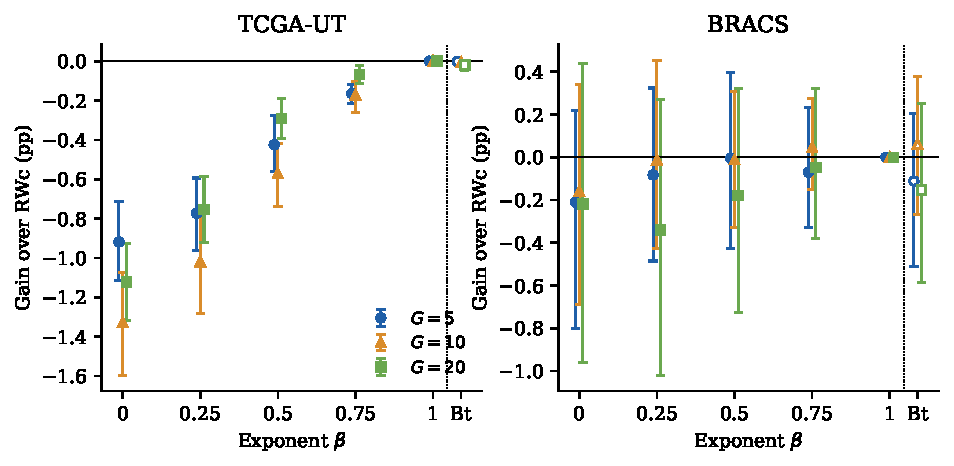
\includegraphics[width=\textwidth]{beta_profile.pdf}
\caption{Compressing the cohort's between-patient spectrum only costs accuracy; the validation-tuned arm returns to the uncompressed spectrum. Paired gain over cohort whitening in percentage points against the exponent $\beta$, with $\beta=1$ being cohort whitening itself and therefore zero by construction. The open markers right of the dotted line are the validation-tuned arm Bt. Error bars show the paired 95\% bootstrap intervals; markers are offset horizontally to separate the patient counts.}
\label{fig:profile}
\end{figure}

\noindent The BRACS profile is flat within its intervals, which span about one point at $\beta=0$ and narrow toward $\beta=1$. Nothing in it separates the exponents, and the widest departure from cohort whitening, $-0.34$ points at $\beta=0.25$ and twenty patients, has an interval from $-1.02$ to 0.27.

\subsection{Spectrum against directions}
\label{sec:decomposition-results}
The oracle arm bounds what the spectrum can contribute, and the bound is small. On TCGA-UT it gains 0.08 points over cohort whitening at five patients (0.03 to 0.13), 0.02 at ten ($-0.01$ to 0.04), and 0.02 at twenty (0.01 to 0.04). Against these values, pool-basis whitening exceeds the oracle arm by 2.58 points at five patients (2.25 to 2.89), 2.00 at ten, and 1.26 at twenty. The gap of 2.66 points between cohort-basis and pool-basis whitening at five patients therefore splits into a spectrum part of 0.028 (0.013 to 0.050) and a direction part of the remaining 97 percent (Figure~\ref{fig:decomposition}). On BRACS the same decomposition is uninformative in absolute terms, because cohort whitening gains nothing there, but the ordering is the same: the oracle arm stays within 0.24 points of cohort whitening at every patient count, while pool-basis whitening exceeds it by 2.96 points at five patients (1.48 to 4.58).

\begin{figure}[htbp]
\centering
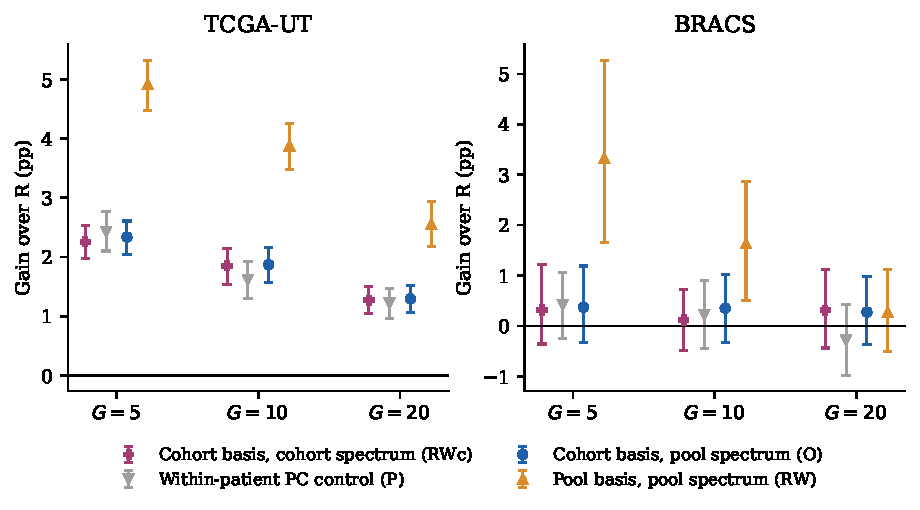
\includegraphics[width=\textwidth]{decomposition.pdf}
\caption{Replacing the cohort's eigenvalues by the pool variances along the same directions moves accuracy by less than a tenth of a point; replacing the directions moves it by two to three points. Paired gains over the real cohort in percentage points at each patient count. Error bars show the paired 95\% bootstrap intervals; markers are offset horizontally within each patient count.}
\label{fig:decomposition}
\end{figure}

\noindent The direction control shows that the between-patient directions are not specific. Whitening along the top within-patient principal components of matched rank, with the cohort eigenvalues attached in rank order, matches cohort whitening on both datasets: the contrast RWc $-$ P is $-0.17$ points at five TCGA-UT patients ($-0.44$ to 0.10), 0.24 at ten, and 0.05 at twenty, and on BRACS it ranges from $-0.12$ to 0.59 points; every interval includes zero. At five TCGA-UT patients the control is in fact the numerically best cohort-only arm in the study, at 64.91 percent against 64.74 for cohort whitening, though the difference is well inside its interval. The two subspaces are not unrelated: their overlap is 0.447 at five patients, ten times the 0.047 expected for a random subspace of rank 120 in 2,560 dimensions (Table~\ref{tab:diagnostics}), so the control shows that a second high-variance cohort subspace whitens equally well, not that an arbitrary subspace would.

\subsection{Diagnostics and validation selection}
\label{sec:diagnostics-results}
The cohort spectrum is over-dispersed in the direction the motivation predicted. The oracle exponent, the slope of $\log v_j$ on $\log\lambda_j$ within a fit, averages 0.816 at five TCGA-UT patients and falls to 0.743 at twenty; on BRACS it averages 0.830 at five patients and approaches one at twenty (Table~\ref{tab:diagnostics}). Every value is below one, so the pool variances along the cohort's directions are indeed less spread than the cohort's own eigenvalues, and no value exceeds one, so the grid's exclusion of $\beta>1$ is not what produced the null result. The cohort subspace also misses a substantial part of the population structure: it contains 69.8 percent of the pool's between-patient variance at five TCGA-UT patients and 57.7 percent on BRACS, rising to 93.8 and 87.6 percent at twenty patients.

\begin{table}[htbp]
\centering
\small
\renewcommand{\arraystretch}{1.15}
\begin{tabular}{@{}lrrrrrr@{}}
\toprule
 & \multicolumn{3}{c}{TCGA-UT} & \multicolumn{3}{c}{BRACS} \\
\cmidrule(lr){2-4}\cmidrule(lr){5-7}
 & $G=5$ & $G=10$ & $G=20$ & $G=5$ & $G=10$ & $G=20$ \\
\midrule
Rank $r=C(G-1)$ & 120 & 270 & 570 & 28 & 63 & 133 \\
Oracle exponent & 0.816 & 0.783 & 0.743 & 0.830 & 0.909 & 0.973 \\
Pool variance in cohort span & 0.698 & 0.845 & 0.938 & 0.577 & 0.760 & 0.876 \\
Subspace overlap with control & 0.447 & 0.544 & 0.641 & 0.394 & 0.454 & 0.491 \\
Overlap of a random subspace & 0.047 & 0.105 & 0.223 & 0.011 & 0.025 & 0.052 \\
\addlinespace
Selected $\beta=0$ & 0 & 0 & 0 & 8 & 10 & 4 \\
Selected $\beta=0.25$ & 0 & 0 & 0 & 5 & 4 & 3 \\
Selected $\beta=0.5$ & 0 & 0 & 0 & 5 & 4 & 7 \\
Selected $\beta=0.75$ & 1 & 2 & 12 & 7 & 2 & 5 \\
Selected $\beta=1$ & 29 & 28 & 18 & 5 & 10 & 11 \\
\bottomrule
\end{tabular}
\caption{The cohort spectrum is over-dispersed, yet validation almost always keeps it on TCGA-UT. The oracle exponent is the within-fit slope of the log pool variance on the log cohort eigenvalue; the pool-variance share and the subspace overlap are defined in Section~\ref{sec:model}; the random-subspace row is the reference value $r/2{,}560$ for the overlap. The first four rows are means over the 30 fits per patient count; the selection rows are counts of those 30 fits.}
\label{tab:diagnostics}
\end{table}

\noindent Validation selection separates the two datasets sharply. On TCGA-UT the tuned arm keeps $\beta=1$ in 29 of 30 fits at five patients and 28 of 30 at ten, so the selection rule almost never departs from cohort whitening, and where it does the departure does not pay: at twenty patients validation prefers $\beta=0.75$ in 12 of 30 fits, and the resulting test contrast is $-0.02$ points, consistent with selection noise rather than with a real benefit. On BRACS the selections spread over the whole grid --- 8, 5, 5, 7, and 5 fits across the five exponents at five patients --- which is what an uninformative validation signal on 24 validation patients produces, and the corresponding test contrast is $-0.11$ points.

The whitening scale absorbs part of the compression without repairing it. On TCGA-UT the flat arm shifts its selected scale factor upward, to 10 in 27 of 30 fits at five patients and to 1 or 10 in 27 to 30 of 30 fits at the larger patient counts, whereas the arms at $\beta\geq0.5$ and the oracle arm select factor 1 in 19 to 24 of 30 fits at five patients and in all 30 at ten and twenty, matching the behaviour of cohort whitening \citep{queisler2026patientDirections}. Flattening the spectrum thus calls for a stronger contraction of the subspace, and the tuning grid supplies it, yet the arm still loses 0.92 points. On BRACS the smallest factor 0.1 is selected in 12 to 18 of 30 fits in every family, the same near-inactive whitening reported for that dataset by \citet{queisler2026bracsMechanism}; the largest factor 100 is selected in at most 2 of 30 fits anywhere.

\section{Discussion}
\label{sec:discussion}
Of the four readings fixed in Section~\ref{sec:evaluation}, the results select the second and the fourth. The tuned arm matches cohort whitening to within 0.02 points at every patient count on TCGA-UT and to within 0.15 on BRACS, and the oracle arm, which replaces the cohort's eigenvalues by the population quantity they estimate, adds at most 0.08 points. The spectrum is therefore not the bottleneck of cohort whitening, and the direction control adds that the specific between-patient directions are not required either.

The null result is not a failure to detect over-dispersion. The diagnostics confirm it: the pool variances along the cohort's directions grow like the 0.74 to 0.82 power of the cohort's eigenvalues, so the sample spectrum is spread more widely than the population one, exactly as the random-matrix argument predicts \citep{marchenko1967,johnstone2001}. What the results show is that this error is inconsequential for the task. Two properties of Equation~\ref{eq:whiten} explain why. The transform depends on the spectrum only through the saturating factors $(1+\kappa\nu_j)^{-1/2}$, and the scale-free normalization of $\kappa$ removes any common factor, so a moderate distortion of the eigenvalue ratios changes the transform far less than it changes the covariance estimate. And the arm that gets those ratios exactly right gains 0.08 points, which caps what any rule in this family could deliver, whether a power law, linear shrinkage \citep{ledoit2004wellconditioned}, or the direction-wise corrections of nonlinear shrinkage \citep{ledoit2020analytical}. Better covariance estimation is a solved problem that this application does not have.

What the cohort lacks is directions. Its rank-120 subspace at five patients contains 70 percent of the pool's between-patient variance, and closing the remaining gap to the pool basis is worth 2.58 points, thirty times the entire spectrum headroom. The same asymmetry holds at ten and twenty patients, and on BRACS, where the cohort subspace holds only 58 percent of the pool variance at five patients and cohort whitening gains nothing at all. This sharpens the conclusion of the preceding studies. Cohort whitening, directional shrinkage \citep{queisler2026directionalShrinkage}, and centre-uncertainty training \citep{queisler2026centreUncertainty} converge at about one to two points not because they estimate the same covariance imprecisely, but because they can only act inside the span that $C(G-1)$ patient deviations reach. A remedy that improves on them must widen that span, which requires between-patient structure from outside the labelled cohort --- unlabelled slides, related cohorts, or a population covariance carried by the feature extractor --- rather than a better-conditioned estimate from inside it.

The direction control refines the mechanism statement of the earlier reports in a way that was not anticipated. Whitening along the top within-patient principal components performs as well as whitening along the between-patient eigenvectors, at matched rank and with the same eigenvalues, on both datasets. The two subspaces overlap by 0.39 to 0.64, far above chance, so this is not evidence that any subspace works; the high-variance directions of patch-level variation within patients and the directions along which patient means differ are partly the same directions. It does mean that the effective description of the remedy is a contraction of a high-variance low-rank subspace estimated from the cohort, and that the between-patient construction, which is the more expensive of the two and needs the patient labels, is not what makes it work.

\section{Limitations}
\label{sec:limitations}
The oracle arm is an oracle for one target, not a maximum over all spectra. It sets each eigenvalue to the pool's between-patient variance along that direction, which is the quantity the cohort eigenvalue estimates, but a spectrum chosen to maximize test accuracy on the same basis could exceed it. Such a search was not run, and the claim that the spectrum contributes 0.08 points is therefore a claim about estimating the intended quantity correctly, not about the best conceivable reweighting of the cohort's directions.

The power family is one-parameter and monotone, so it cannot represent a correction that moves small and large eigenvalues in opposite directions, as nonlinear shrinkage does. That family was not fitted; the argument against it rests on the oracle bound, which applies to any fixed-basis spectrum aimed at the pool variances. The grid stops at $\beta=1$, and exponents above one were not tested. The oracle exponents, all between 0.74 and 0.97, point away from that region, but this is a diagnostic rather than a test, and the diagnostic summarizes a scattered relation by a single slope.

The direction control is matched in rank and in eigenvalues but overlaps the cohort basis substantially, so it separates the between-patient construction from high-variance directions in general, and not from arbitrary directions. A perturbation matched per direction, for example a random subspace drawn inside the span of the pool covariance, was not run. All arms reuse the three evaluation splits of the source studies, so they share test patients with every earlier comparison in this series, and repeated use of these partitions inflates the chance that some arm appears to work by selection alone. On BRACS the host remedy gains nothing, so the spectrum contrasts there test a modification of an inactive treatment, and the intervals, which span roughly one point for the power arms and three for the direction contrast, admit effects that the design cannot resolve. The results are conditional on frozen Virchow2 features, multinomial logistic regression, 160 patches per class, and the two cohorts studied.
